\documentclass[12pt]{article}
% Load packages
\usepackage{url}  % Formatting web addresses
\usepackage{ifthen}  % Conditional
\usepackage{multicol}   %Columns
\usepackage[utf8]{inputenc} %unicode support
\usepackage{amsmath}
\usepackage{amssymb}
\usepackage{epsfig}
\usepackage{epstopdf}
\usepackage{graphicx}
\usepackage[margin=0.1pt,font=footnotesize,labelfont=bf]{caption}
\usepackage{setspace}
%\usepackage{longtable}
\usepackage{colortbl}
%\usepackage{palatino,lettrine}
%\usepackage{times}
%\usepackage[applemac]{inputenc} %applemac support if unicode package fails
%\usepackage[latin1]{inputenc} %UNIX support if unicode package fails
\usepackage[wide]{sidecap}
%\usepackage[authoryear,round,comma,sort&compress]{natbib}
\usepackage[square,sort,comma,numbers,sort&compress]{natbib}
%\usepackage[authoryear,round]{natbib}
\usepackage{supertabular}
\usepackage{simplemargins}
\usepackage{fullpage}
\usepackage{comment}
\usepackage{lineno}
%\usepackage{chicago}
\usepackage{textcomp}
\usepackage{multirow}
\usepackage{amsmath}
\usepackage[linesnumbered,lined,boxed,commentsnumbered]{algorithm2e}
\DeclareMathOperator*{\argmin}{\arg\!\min}

\usepackage{algorithm2e}
\usepackage{algpseudocode}
%\usepackage[space]{cite}
\urlstyle{rm}

%\textwidth = 6.50 in
%\textheight = 9.5 in
%\oddsidemargin =  0.0 in
%\evensidemargin = 0.0 in
%\topmargin = -0.50 in
%\headheight = 0.0 in
%\headsep = 0.25 in
%\parskip = 0.15in
%\linespread{1.75}
\doublespace

%\bibliographystyle{chicago}
\bibliographystyle{plos2009}

\makeatletter
\renewcommand\subsection{\@startsection
	{subsection}{2}{0mm}
	{-0.05in}
	{-0.5\baselineskip}
	{\normalfont\normalsize\bfseries}}
\renewcommand\subsubsection{\@startsection
	{subsubsection}{2}{0mm}
	{-0.05in}
	{-0.5\baselineskip}
	{\normalfont\normalsize\itshape}}
\renewcommand\section{\@startsection
	{subsection}{2}{0mm}
	{-0.2in}
	{0.05\baselineskip}
	{\normalfont\large\bfseries}}
\renewcommand\paragraph{\@startsection
	{paragraph}{2}{0mm}
	{-0.05in}
	{-0.5\baselineskip}
	{\normalfont\normalsize\itshape}}
\makeatother

%Review style settings
%\newenvironment{bmcformat}{\begin{raggedright}\baselineskip20pt\sloppy\setboolean{publ}{false}}{\end{raggedright}\baselineskip20pt\sloppy}

%Publication style settings

% Single space'd bib -
\setlength\bibsep{0pt}

\renewcommand{\rmdefault}{phv}\renewcommand{\sfdefault}{phv}
\newcommand{\norm}[1]{\left\lVert#1\right\rVert}

% Change the number format in the ref list -
\renewcommand{\bibnumfmt}[1]{#1.}

% Change Figure to Fig.
\renewcommand{\figurename}{Fig.}

% Begin ...
\begin{document}
\begin{titlepage}
{\par\centering\textbf{\Large {Dynamic Modeling of Human Complement System using Reduced Ordered Models}}}
\vspace{0.05in}
{\par \centering \large{Adithya Sagar, Wei Dai, Mason Minor, and Jeffrey D. Varner$^{*}$}}
\vspace{0.10in}
{\par \centering {School of Chemical and Biomolecular Engineering}}
{\par \centering {Cornell University, Ithaca NY 14853}}
\vspace{0.1in}
{\par \centering \textbf{Running Title:}~Dynamic Modeling of Human Complement System using Reduced Ordered Models}
\vspace{0.1in}
{\par \centering \textbf{To be submitted:}~\emph{???????}}
\vspace{0.5in}
{\par \centering $^{*}$Corresponding author:}
{\par \centering Jeffrey D. Varner,}
{\par \centering Professor, School of Chemical and Biomolecular Engineering,}
{\par \centering 244 Olin Hall, Cornell University, Ithaca NY, 14853}
{\par \centering Email: jdv27@cornell.edu}
{\par \centering Phone: (607) 255 - 4258}
{\par \centering Fax: (607) 255 - 9166}
\end{titlepage}
\date{}
\thispagestyle{empty}
\pagebreak
%%%%%%%%%%%%%%%%%%%%%%%%%%%%%%%%%%%%%%%%%%%%%%%%%%%%%%%%%%%%%%%%%%%%%%%%%%%%%%%%%%%%%%%%%%%%%%%%%%%%%%%%%%%
%%%%%%%%%%%%%%%%%%%%%%%%%%%%%%%%%%%%%%%%%%%%%%%%%%%%%%%%%%%%%%%%%%%%%%%%%%%%%%%%%%%%%%%%%%%%%%%%%%%%%%%%%%%
\section*{Abstract}
Fill me in.


%We further tested the predictive power of the coagulation model parameters against data not used in training, and found good agreement between simulations and experimental measurements. Lastly, we tested the performance of DOPS on commonly used test functions for global optimization and on published biochemical parameter estimation benchmark problems. For the wide range of problems that we considered, DOPS outperformed other meta-heuristic approaches despite a limited number of function evaluations.

\vspace{0.1in}
{\noindent \textbf{Keywords:}~Biochemical engineering, systems biology, reduced order models, complement system}

% Extra abstract
% Mathematical modeling of biological systems with multiple feed back loops is one such area where parameter estimation is a difficult non-linear optimization problem. This difficulty is further compounded when dealing with parameter vectors of high dimensions.

%In this study, we present the dynamically dimensioned particle
%a novel meta-heuristic approach that combines a variant of particle swarm optimization (PSO) along with dynamically dimensioned search (DDS) to obtain near optimal solutions of high dimensional biochemical networks within a relatively few function evaluations.
%We use a particle swarm optimization technique that uses multi-swarms to generate candidate vectors which are then greedily updated using DDS by dynamically varying the perturbed parameter dimensions. We tested this algorithm (25 trials with 4000 function evaluations in each trial) on a biochemical network of coagulation (148 parameters and 92 species) and compared it's performance against other meta-heuristics like Differential Evolution (DE), Particle Swarm Optimization (PSO), Simulated Annealing (SA) and also against DDS alone. The new algorithm outperforms all the other meta-heuristics on the coagulation model. The parameter vectors obtained using this approach fit the experimental data well and also make accurate enough predictions on unseen experimental data. We also performed this comparison on commonly used test functions (Ackley and Rosenbrock) for global optimization and found the same behavior. Further we used two recently published benchmark problems, a genome wide kinetic model with 1759 parameters and a metabolic model of Chinese Hamster Ovary cells with 117 parameters to evaluate the performance of our approach. We  surprisingly performed well on these benchmarks and obtained the nominal parameter vector with just 4000 function evaluations in both cases.

\pagebreak

\setcounter{page}{1}

% Uncomment in production -
\linenumbers


\section*{Introduction}
The introduction has three paragraphs (introduction no longer than 3 pages):
\begin{enumerate}
	\item{\textbf{First~paragraph}: Introduce human complement system, history, role in adaptive/innate immunity. }
	\item{\textbf{Second~paragraph}: Introduce mathematical models of complement system, current place in the field, our work was not possible without xyz who pioneered abc. Address shortcomings in the field .}
	\item{\textbf{Third~paragraph}: In this study, [Repeat the abstract with some additional detail]. Taken together, [killer statement].}
\end{enumerate}

% Extra text from the introduction -
%With the capacity to construct very large models using various mathematical formalisms \cite{chen2009input,tasseff2011modeling,luan2007computationally,mo2007genome,orth2011comprehensive,karr2012whole,buchel2013path2models,smallbone2010towards}, more often than not,

%this algorithm (25 trials with 4000 function evaluations in each trial) on a biochemical network of coagulation (148 parameters and 92 species) and compared it's performance against other meta-heuristics  The new algorithm outperforms all the other meta-heuristics on the coagulation model. The parameter vectors obtained using this approach fit the experimental data well and also make accurate enough predictions on unseen experimental data. We also performed this comparison on  and found the same behavior. Further we used two recently published benchmark problems, a genome wide kinetic model with 1759 parameters and a metabolic model of Chinese Hamster Ovary cells with 117 parameters to evaluate the performance of our approach. We  surprisingly performed well on these benchmarks and obtained the nominal parameter vector with just 4000 function evaluations in both cases.
%took into cognizance the fact that it may not be necessary to obtain the exact solution for high dimensional biological systems and that good enough solutions can be quickly obtained without expending a lot of objective function evaluations. Hence our current approach uses the power of population based heuristics along with DDS to obtain near optimal or good solutions. Though in theory we can combine any meta-heuristic with DDS, for the current purpose we used Particle Swarm Optimization (PSO). PSO unlike Genetic Algorithm (GA) or Differential Evolution (DE) does not have complex operations like cross over, mutation or recombination. It is simple to use and does not have a lot of parameters associated with other heuristics. However PSO is known to rapidly converge to a local optimum and thus several variants \cite{peer2003using,zhan2009adaptive,li2007fast} have been developed of which Multi swarm particle swarm optimization approaches (MLSPSO) \cite{zhao2008dynamic,liang2005dynamic} are one of the effective ones. We used MLSPSO to preclude bad regions of search and thereafter search within these regions using DDS.

\clearpage

\section*{Results}

The results are presented in \textbf{past~tense}. Each paragraph starts with a statement of the result in that paragraph in active voice.
Each results paragraph ends with a Taken together type statement followed by a link statement e.g., Next we considered etc. When referring to figures, state what the figures shows (Fig. ZZ).


\clearpage

%As the dimensionality of  increases, the search region gets widened and thus the problem becomes more challenging.
%

\section*{Discussion}

The discussion has three (sometimes four) paragraphs:
\begin{enumerate}
	\item{\textbf{First~paragraph}: Present a modified version of the last paragraph of the introduction. In this study, [...]. Taken together, [killer statement]}
	\item{\textbf{Second~paragraph}: Contrast the key findings of the study with other computational/experimental studies}
	\item{\textbf{Third~paragraph}: Present future directions. If you had more time, what would like to do? Highlight the key shortcomings of the approach and how will we address them in the future.
	In this case, we will have a scaling issue if we extend to genome scale. We should extend to dynamic cases, and we need to experimentally validate the findings. }
\end{enumerate}

\clearpage

\section*{Materials and Methods}

\begin{enumerate}
	\item{\textbf{Model~formulation}: Present the reduced order modeling approach of the human complement network, . Outline parameter estimation, and state all parameter assumptions, sensitivity analysis}
\end{enumerate}

\clearpage

%Need to talk more about biochemical benefits and importance for of biochemical problems

\section*{Acknowledgements}
This study was supported by an award from [FILL ME IN].
\clearpage


\bibliography{References_v1}

\clearpage

% Figures and captions go here ...
%\begin{figure}[ht]
%\centering
%\includegraphics[width=1.00\textwidth]{./figs/<Filename>.pdf}
%\caption{Captiontext goes here}
%}\label{fig:<label_name>}
%\end{figure}
\begin{figure}[h]
\centering
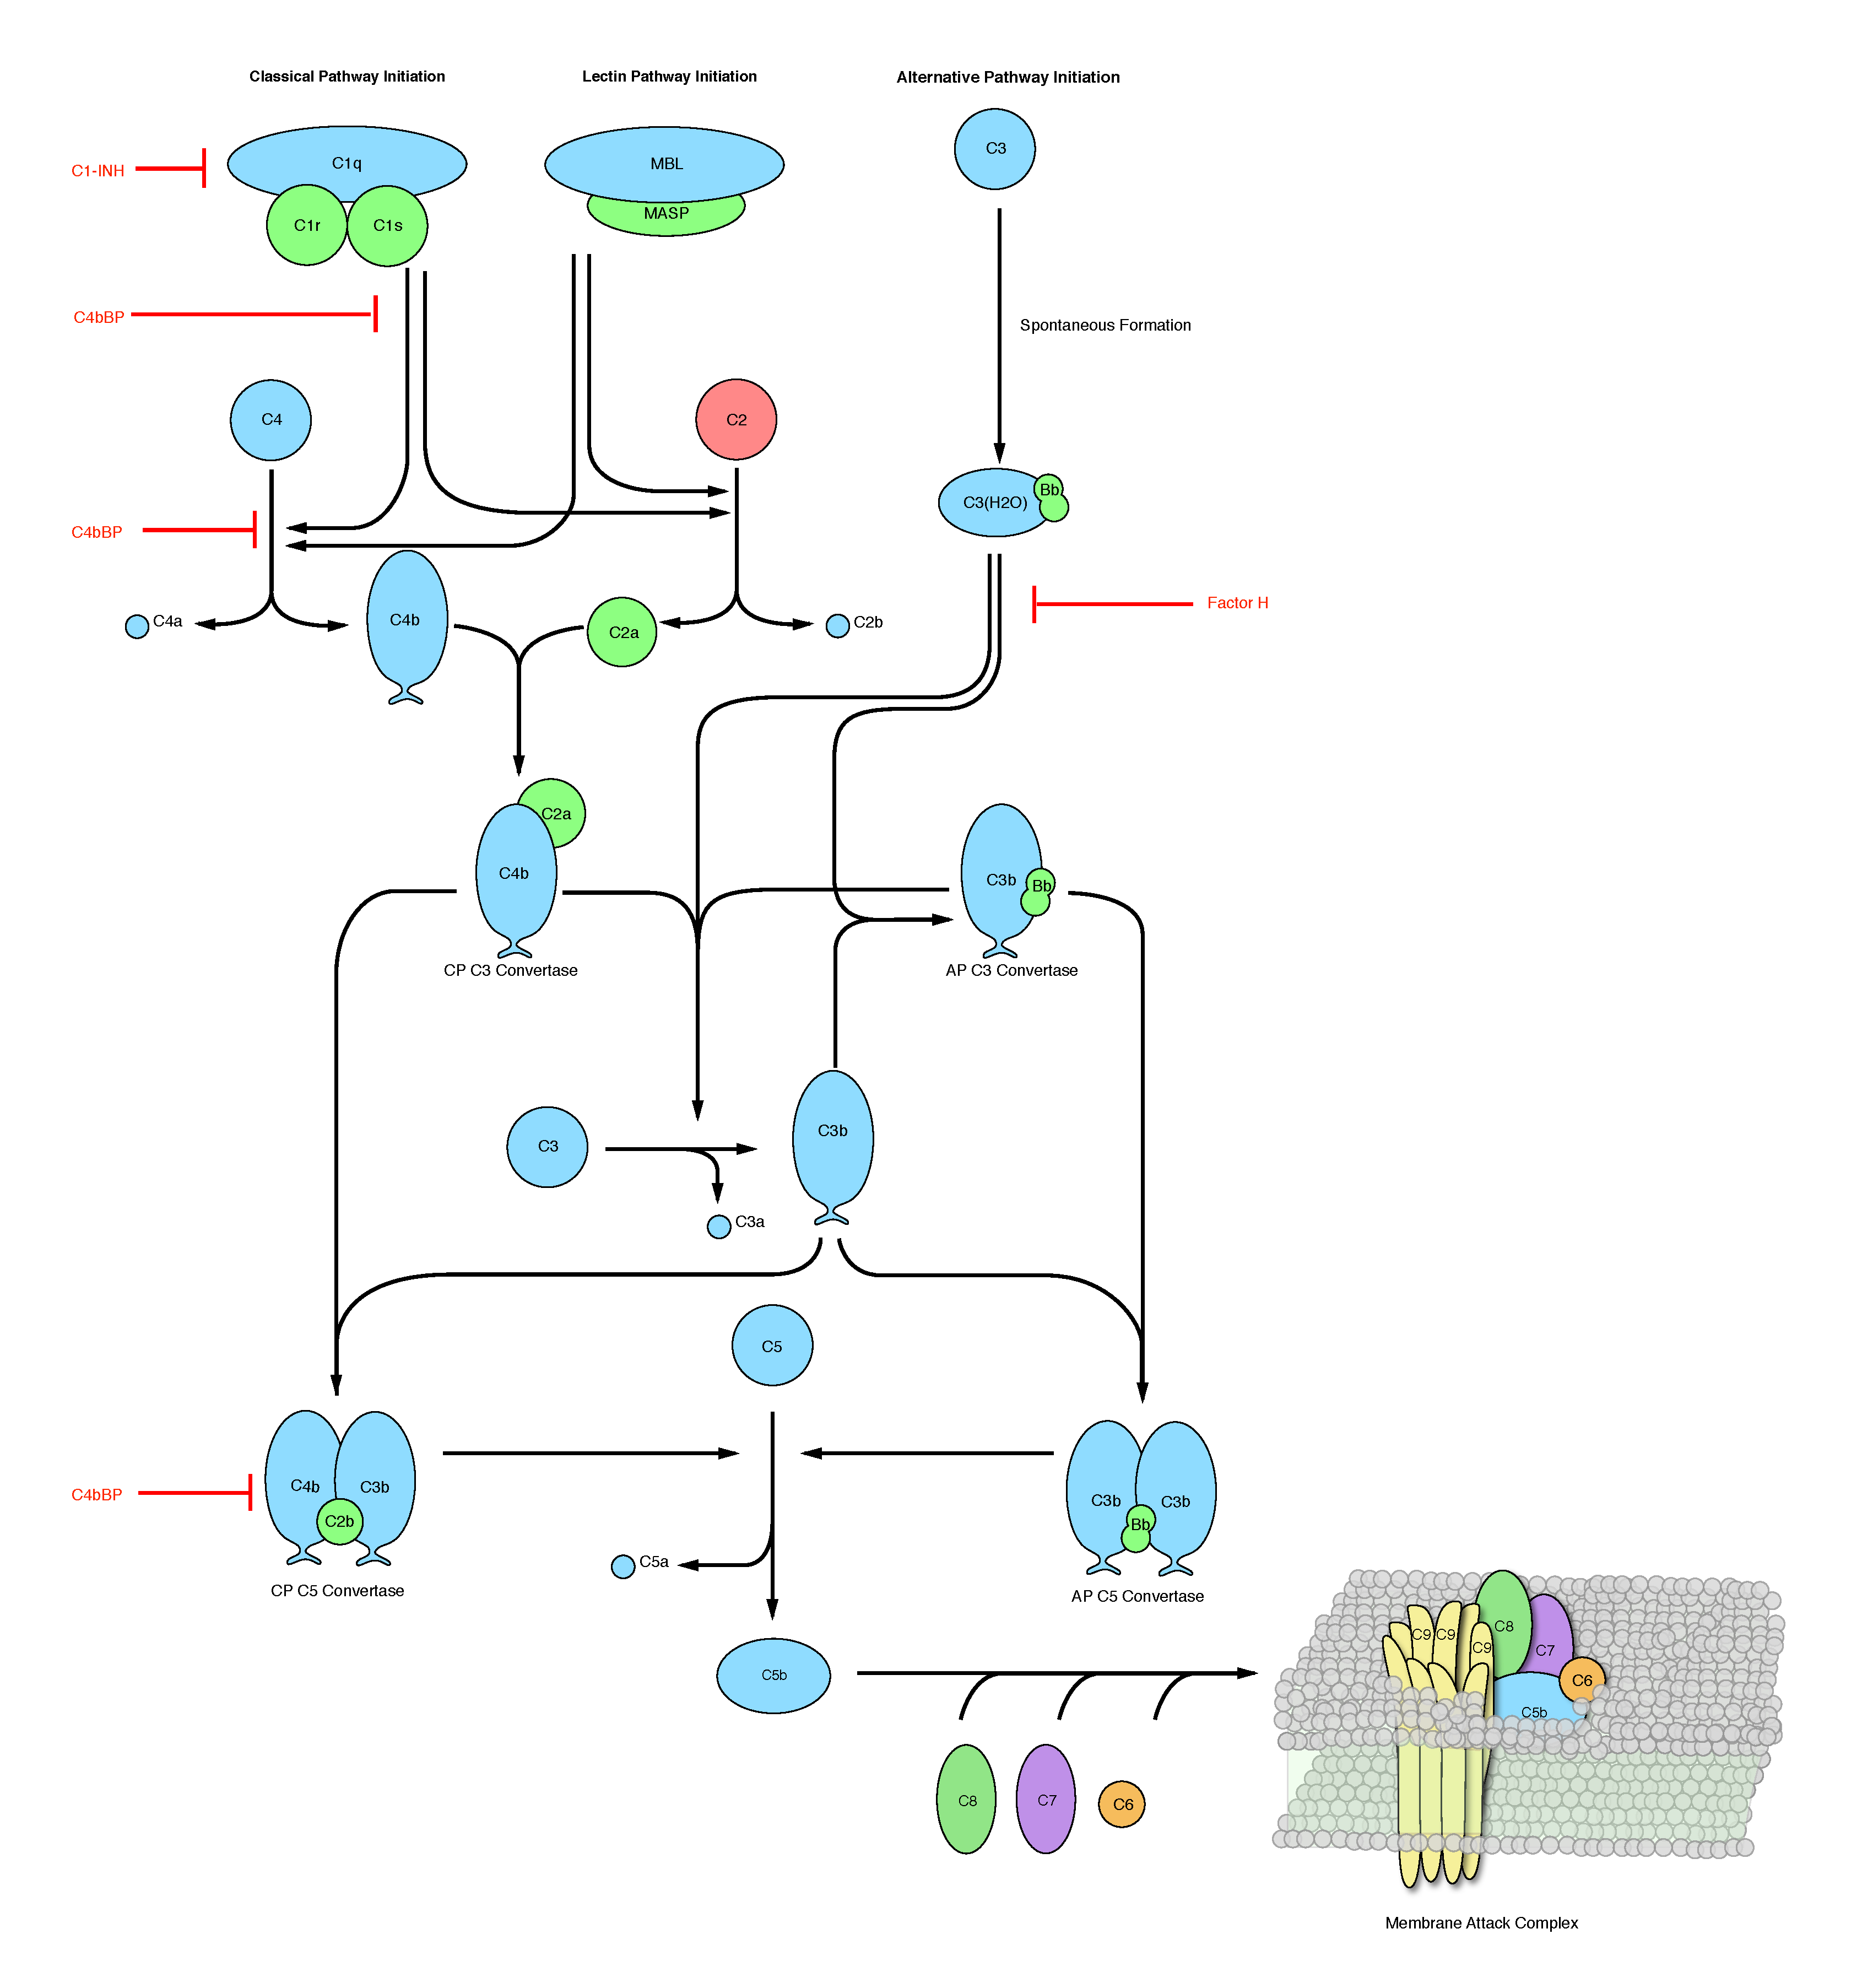
\includegraphics[width=1.0\textwidth]{./Figures/ComplementSystemSchematic_v1.pdf}
\caption{The biochemical reactions of the complement system.
}\label{fig1-schematic}
\end{figure}



\clearpage

% Supplemental figures -
% Set the S-
\renewcommand\thefigure{S\arabic{figure}}
\renewcommand\thetable{T\arabic{table}}
\renewcommand\thepage{S-\arabic{page}}
\renewcommand\theequation{S\arabic{equation}}

% Reset the counters -
\setcounter{equation}{0}
\setcounter{table}{0}
\setcounter{figure}{0}
\setcounter{page}{1}


% Supplemental figures go here ...
%\begin{figure}[ht]
%\centering
%\includegraphics[width=1.00\textwidth]{./figs/<Filename>.pdf}
%\caption{Captiontext goes here}
%}\label{fig:<label_name>}
%\end{figure}

\end{document}
